\section{Phase 3: Comparison to Other Solvers}
\label{phase3}

\subsection{Goal}
At the end of Phase 2 in Section \ref{phase2}, the implementation for our \aspop{} solver was considered final; This last phase tests how it compares to some existing solvers (namely \textsc{blast} and Minimap) in terms of \textit{output quality}\footnote{As with Phase 1 in Section \ref{phase1}, quality is defined in terms of \textit{F-measure} $=  2\cdot{}precision\cdot{}recall/(precision+recall)$.} and runtime in much the same way as in phase~1.

\textbf{Test 1} represents our primary focus on the use case of an \aspop{} solver in the context of viral genome assembly. Here, desirable \glspl{solution} only come from overlapping regions in the \glspl{source genome}; Only through the discovery of these `true' overlaps can the resulting assembly graph reconstruct these source genomes correctly. As such, the data set selected to represent this use case contains a mix of 5 viral strains. Overlaps found \textit{between} strains are not considered `true', instead counting as false positives and contributing to a diminished measure of precision.

\textbf{Test 2} compares the performance of our \aspop{} solver when applied to human DNA; The intention of this test is to check how runtime and output quality change when the solver is applied to a new type of data set with different properties.

\subsection{Experimental Design}

For each of the two tests, our \aspop{} solver, \textsc{blast} and Minimap were run on the data set sequentially. Many variations of this experiment are conceivable under these conditions, but for our purposes it was most interesting to test the performance of our system in conditions that were found in phase~1 to be conducive to finding the highest-quality solutions set for the purpose of viral genome assembly. As such, runs were done with error rate limit (\bfit{e}) $=$ 1.2\% and threshold overlap length (\bfit{t}) $=$ 80.

All solvers were run on a cluster computer of 24~Intel\textsuperscript{\textregistered} Xeon\textsuperscript{\textregistered} E52620-0s running at~2.00~GHz with 252~GB of storage. Each process was given 10~threads and sufficient free logical cores to run under negligible CPU contention.

The 5-mix of viral genomic data is taken from HXB2 (accession number K03455), available at the NCBI Reference database~\cite{ncbi}. It consists of a sample of 80,000 reads (approximately 2000x coverage) with most reads being of length 250bp.

The human DNA data is taken from Nisk.org's \textit{genome in a bottle} (Individual NA12878)~\cite{genomeinabottle}. Paired-end reads are 2x15 base-pairs at~30x coverage, but with \gls{read} ends truncated of extremely low confidence symbols (resulting in most reads being of length circa 150bp). These reads are taken from a 40,000bp-long subsequence of the MHC region, chromosome~6, base pairs 32,400,000~-~32,800,000.

\subsection{Results}\subsubsection{Viral Genome Data}
\label{p3_viral}

Figure \ref{fig:viral_timespace} shows the properties of the runs for all three solvers, such as the runtime\footnote{Note that runtime is measured \textit{cumulatively} for all running threads in all cores, while wall time is not. This means a well-parallelized program will have a long runtime, but short wall time.} (in terms of user time $+$ system time\footnote{`User time' refers to CPU time spent in user-mode code (outside the kernel) within the process. `System time' refers to CPU time spent in the kernel within the process.}), as well as the total elapsed `wall time' (real-world duration between start and finish of the execution). The peak space\footnote{Similar to runtime, memory usage can also be inflated with response to increased parallelism, as memory of all cores is counted together.} in memory used is also shown.

The Venn diagram given in Figure \ref{fig:viral_venn} shows the \textit{universe} of all unique overlap \glspl{solution} found between all three solvers; Solutions within the \textit{ground truth} set are also shown. Intuitively, a perfect solver's solution set would be equivalent to the ground truth set; Each excluded true solution decreases recall, and each included false solution decreases precision. 

Figure \ref{fig:prec_rec_f_p3} shows the values of recall, precision and \textit{f-measure} for all three solution sets with respect to the ground truth set.

\begin{figure}
\centering
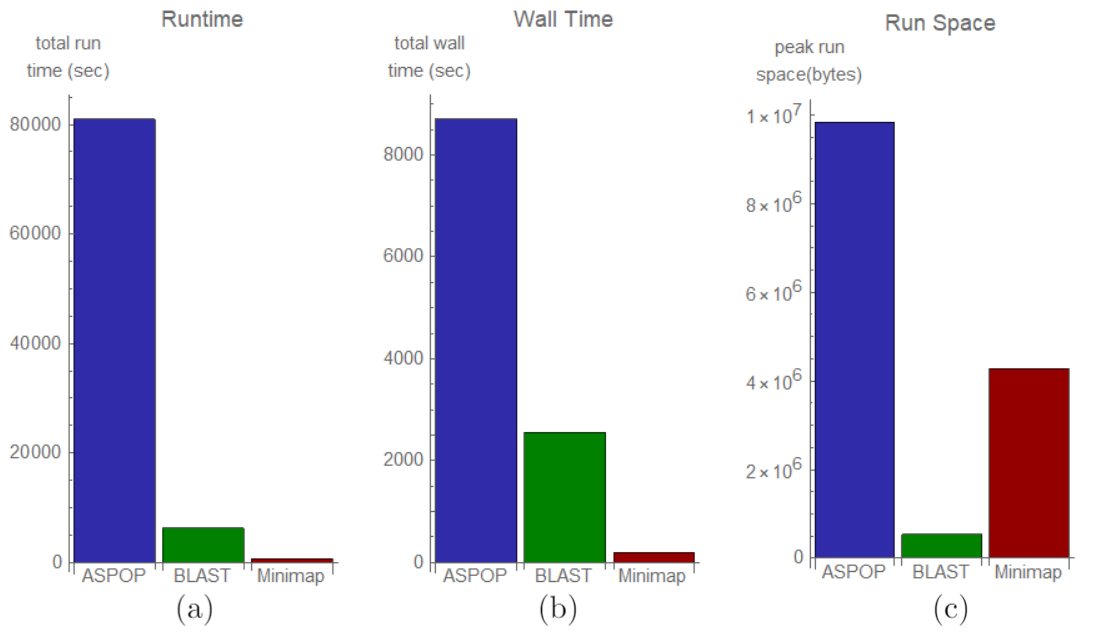
\includegraphics[width=0.85\linewidth]{images/time_space_v.png}
\caption[Time and space usages for runs of three \aspop{} solvers on a moderate data set containing a 5-strain mix of viral strains.]{Time and space usages for runs of three \aspop{} solvers on a moderate data set containing a 5-strain mix of viral strains.\\(a) Runtime of the solver in terms of system and user time in seconds\footnotemark{}.\\(b) Elapsed time as perceived externally in seconds.\\(c) Peak space required during solve in kb.}
\label{fig:viral_timespace}
\end{figure}

\FloatBarrier
\footnotetext{In the previous sections we have used nanosecond-granularity for time measurements, as they were made by a custom \aspop{} benchmarker able to measure time taken by components separately. For this test, we rely on linux's \url{/usr/bin/time} output, which uses second-granularity.}


\begin{figure}
\centering
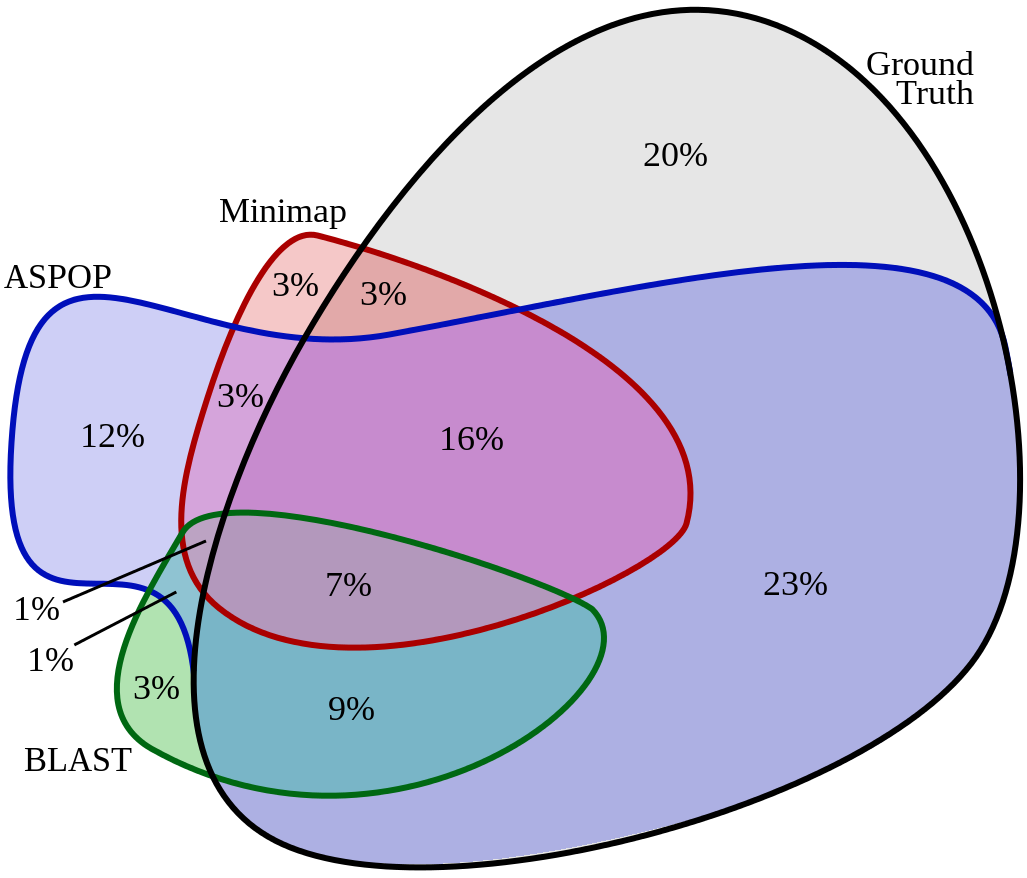
\includegraphics[width=0.55\linewidth]{images/viral_venn.png}
\caption[Venn diagram of solutions common between our \aspop{}, \textsc{blast} and Minimap against the \textit{ground truth} set for for a 5-strain viral mix data set]{Venn diagram of solutions found from a moderate 5-strain viral genome mix using our \aspop{} solver (blue), \textsc{blast} (green), Minimap (red) and the \textit{Ground Truth} (gray). Regions are labeled with the percentage of total solutions found, and are not necessarily to exact scale. Regions whose values round to $< 1\%$ of solutions are not labeled.}
\label{fig:viral_venn}
\end{figure}

\begin{figure}
\centering
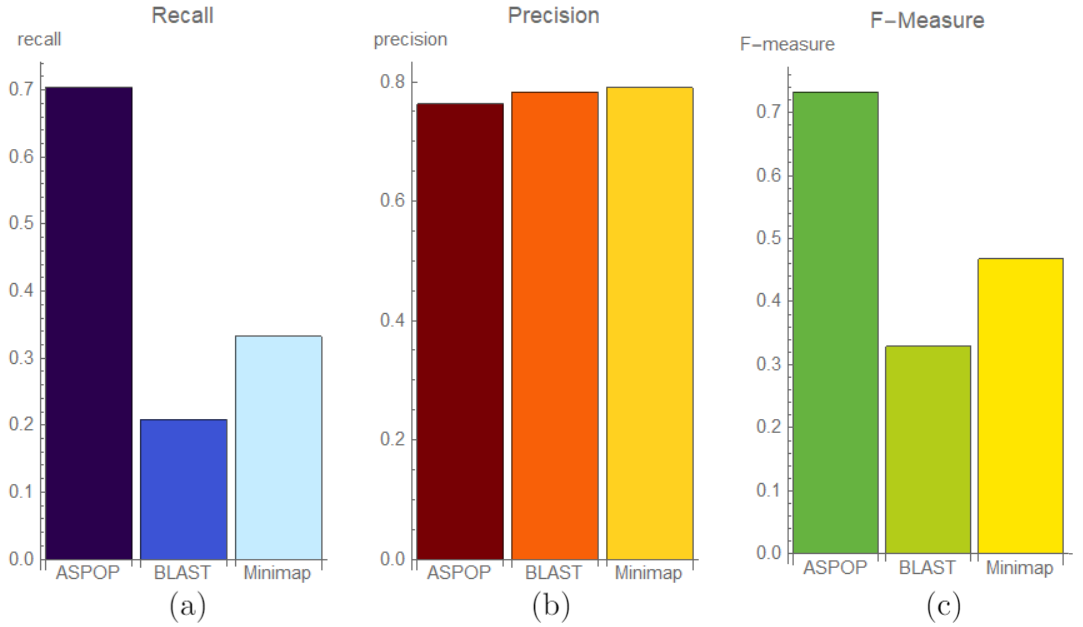
\includegraphics[width=0.9\linewidth]{images/prec_rec_f_p3.png}
\caption[Recall, precision, and f-measure for our \aspop{} solver, \textsc{blast} and Minimap running on a moderate 5-strain mix of viral data.]{Plots of (a) Recall (b) Precision and (c) F-measure for our \aspop{} solver, \textsc{blast} and Minimap running on a moderate 5-strain mix of viral data.}
\label{fig:prec_rec_f_p3}
\end{figure}


% \FloatBarrier


\subsubsection{Human Genome Data}
As in Section \ref{p3_viral} above, Figure \ref{fig:human_timespace} plots values\footnote{As in the previous section, the values of runtime and peak space are sensitive to parallelism. These solvers are parallelized to different degrees so it is important to interpret these measures in the context of wall time to gain a sense of the parallelism influencing the other values.} of runtime, wall time and peak space usage; In this experiment, the solvers were set on a data set containing \glspl{read} from human DNA.

Figure \ref{fig:human_venn} presents a Venn diagram of the \textit{universe} of \glspl{solution} found by all three solvers. Note that unlike the viral experiment, this data set has no known \textit{ground truth} set, as this is not simulated data under our control. As such, this diagram can only hint at the relationships between these solution sets, such as in which ways they are similar, different or how the size\footnote{\textsc{blast}, for instance, can output the same solution numerous times. Only \textit{unique} solutions are considered for these experiments.} between solution sets compare.



\begin{figure}
\centering
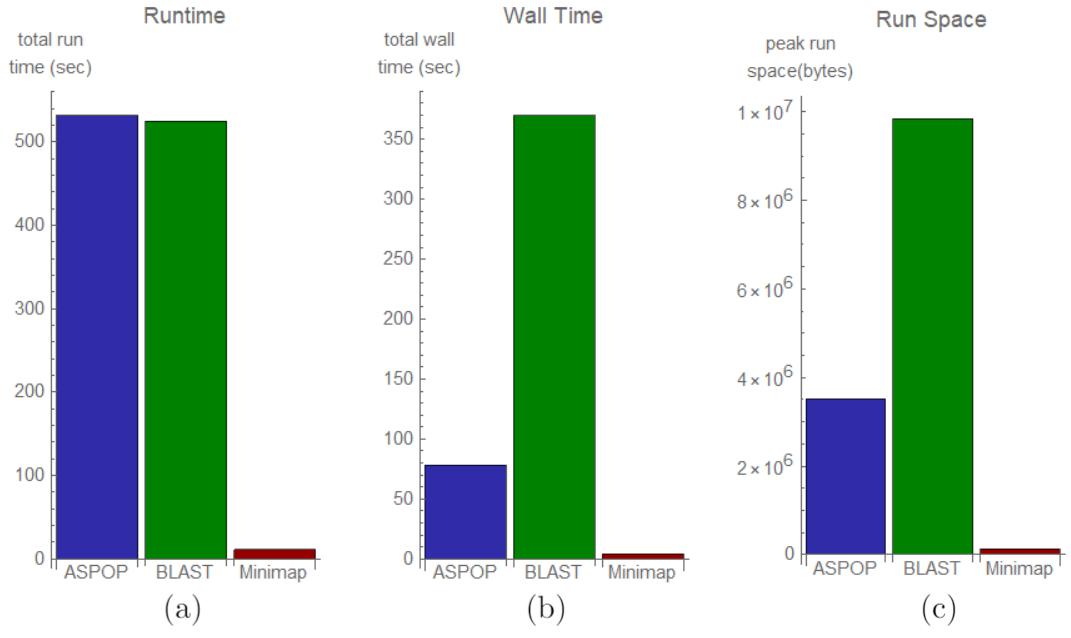
\includegraphics[width=0.9\linewidth]{images/time_space_h.png}
\caption[Time and space usages for runs of three \aspop{} solvers on a moderate data set containing a sample of human DNA]{Time and space usages for runs of three \aspop{} solvers on a moderate data set containing a sample of human DNA.\\(a) Runtime of the solver in terms of system and user time in seconds.\\(b) Elapsed time as perceived externally in seconds.\\(c) Peak space required during solve in kb.}
\label{fig:human_timespace}
\end{figure}

\begin{figure}
\centering
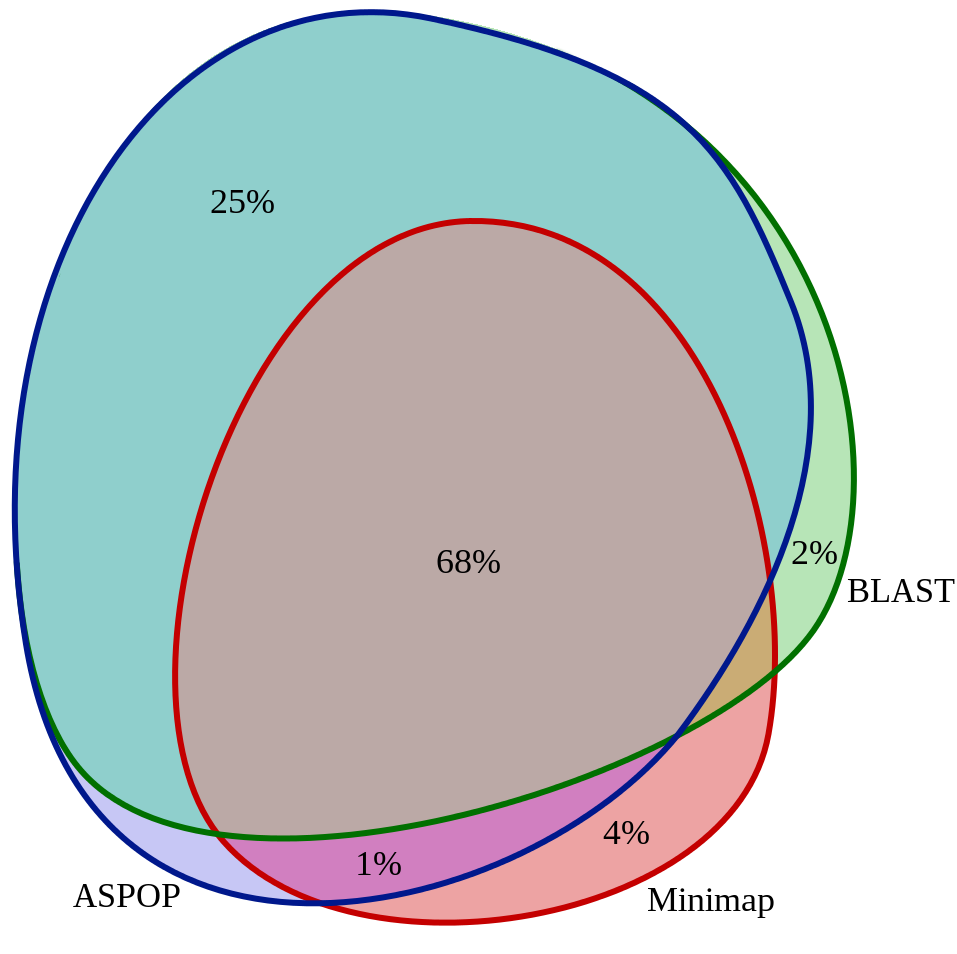
\includegraphics[width=0.5\linewidth]{images/human_venn.png}
\caption[Venn diagram of solutions common between our \aspop{}, \textsc{blast} and Minimap for for a data set of human DNA]{Venn diagram of solutions found from a small data set of human DNA using our \aspop{} solver (blue), \textsc{blast} (green) and Minimap (red). Regions are labeled with the percentage of total solutions found, and are not necessarily to exact scale. Regions whose values round to $< 1\%$ of solutions are not labeled.}
\label{fig:human_venn}
\end{figure}





\subsection{Observations}

Much can be ascertained about our \aspop{} solver, as well as its competitors, from the results of just these two experiments. It is immediately striking that Minimap is \textit{blazingly-fast} despite the fact that it didn't effectively make use of all 10 worker threads. Section \ref{fullmhc} shows that in a larger data set, Minimap's speed superiority becomes even more pronounced. In both cases, Minimap wrote \glspl{solution} in somewhere around 2\% of the time taken for our \aspop{} solver. However, overall, Minimap missed the largest percentage of solutions of all three solvers.

\textsc{blast} seemed to struggle with the human data, experiencing a spike in the wall time as well as peak run space. As this was not the case with the viral data, it seems likely that this is a result of blast struggling with the \textit{genome length}; This is a property with a large value for the human data set \textit{relative} to properties of the viral data set. \textsc{blast} consistently made the poorest use of parallelism, using an average of 230\% of CPU time even with 10 threads and an abundance of cores.

Our \aspop{} solver was generally the slowest solver of the three, specifically for the heftier viral data set. Our \aspop{} solver also had the largest space peak usage. However,  this is likely attributed to its thorough use of the available worker threads in tandem; With space requirements scaled to effective CPU usage, our solver had a smaller peak space usage than \textsc{blast} (and also Minimap in the human data experiment). On the other hand, our solver had the superior \textit{output quality}, represented by the F-measure for the viral experiment, where the \textit{ground truth} set was known. Although solvers were largely indistinguishable in terms of precision, the \aspop{} solver had the highest recall by far. This is almost certainly a direct result of the \gls{suffix filter} algorithm being \textit{exact}, instead of based on heuristics as with the other solvers.

For the \aspop{}, the choice of \bfit{e}$=1.2\%$ was optimal for the purpose of viral genome assembly. This might not necessarily be the case for the other solvers, lending credence to the notion that a user could achieve similar output quality to our solver using, for instance, Minimap but running it with more \textit{lenient} parameters (higher \bfit{e} or lower \bfit{t}); Minimap certainly has the time to spare for finding extra solutions. More work is needed to see if this holds. From what we know so far, it can however be presumed that running any solver with relaxed parameters results in decreased precision. For this reason, beating our solver's F-measure requires not only increased recall, but increased recall \textit{outweighing} the expected decreased precision.









\subsubsection{A Note about Runtime and Peak Run Space}
\label{note:runtime_runspace}

It is immediately apparent that the \aspop{} solver is the slowest; To make matters worse, for this experiment the \textsc{blast} solver had no choice but to find overlaps below the \textit{overlap length threshold} \bfit{t}, (As this is not an exposed parameter for \textsc{blast}) and to discard\footnote{In this decision there was a degree of compromise. If we kept the below-threshold overlaps we risked producing a \textsc{blast} solution set utterly incomparable to our \aspop{} solver's solution set. Alternatively, we could have removed the short solutions to better understand the sufficiently-long solutions that \textsc{blast} \textit{does} find. We concluded that the former option was the lesser of two evils.} them from the solution set. This was done as it is known from phase~1 of the experiments that short overlaps are undesirable even in ideal circumstances. The same can be said for the \textit{error rate limit} parameter \bfit{e} for Minimap, which is also not an exposed parameter for that solver; For both of the other solvers, this means that they are using time and space to find solutions that they are better off without (for the sake of this experiment at least). Unfortunately their natures are such that they cannot find their good solutions without finding these bad ones also. Thus, the runtimes and peak space measures for this phase's experiments should be taken with a grain of salt.

\FloatBarrier

